The previous chapters considered how to design recoverable software assuming various latencies for persist barriers.
However, the memory system implementation remained unspecified, and ultimately will determine performance.
The remainder of this thesis in turn investigates programming interfaces for persistent memory and how the interface might affect system performance.

This chapter motivates and defines \emph{memory persistency}, a framework for reasoning about and enforcing the order of persist operations.
The following chapters propose and evaluate example persistency models.
Refer to Section~\ref{sec:Background:MemoryConsistency} for a discussion of memory consistency and consistency models.

\section{Introduction}
\label{sec:Persistency:Intro}

Emerging nonvolatile memories (NVRAM) promise high performance recoverable systems.
These technologies, required as replacements for Flash and DRAM as existing technologies approach scaling limits \cite{Lee09}, pair the high performance and byte addressability of DRAM with the durability of disk and Flash memory.
Future systems will place these devices on a DRAM-like memory bus, providing systems with throughput similar to DRAM, yet recoverability after failures.

However, ensuring proper recovery requires constraints on the ordering of NVRAM writes.
Existing DRAM interconnects lack the interface to describe and enforce write ordering constraints; ordering constraints that arise from memory consistency requirements are usually enforced at the processor, which is insufficient for failure tolerance with acceptable performance.
Recent work has suggested alternative interfaces to enforce NVRAM write order and guarantee proper recovery, for example durable transactions and persist barriers \cite{Volos11, Condit09}.
While intuitive and suitable to specific applications, I wish to investigate a more general framework for reasoning about NVRAM write ordering including mechanisms for expressing write constraints that are independent of specific concurrency control mechanisms.

Instead, I recognize that the problem of constraining NVRAM write concurrency strongly resembles memory consistency.
Memory consistency restricts the visible order of loads and stores (equivalently, allowable visible memory states) between processors or cores, allowing operations to reorder so long as expected behavior is guaranteed.
Memory consistency models provide an interface and set of memory order guarantees for the programmer, but separate the implementation; several distinct implementations may fulfill the same memory consistency model, allowing sophisticated optimization (e.g., speculation \cite{Blundell09,Wenisch07,Ceze07,Gniady99,Ranganathan97}).
Relaxing the memory consistency model places an additional burden on the programmer to understand the model and insert the correct annotations, but often allows greater performance.

I introduce \emph{Memory Persistency}, a framework motivated by memory consistency to provide an interface for enforcing the order in which NVRAM writes become durable, an operation we refer to as a ``persist'' (as in previous chapters).
Memory persistency prescribes the order of persist operations with respect to one another and loads and stores, and allows the programmer to reason about guarantees on the ordering of persists with respect to system failures.
The memory persistency model relies on the underlying memory consistency model and volatile memory execution to define persist ordering constraints and the values written to persistent memory.

In the following chapters, I define memory persistency, describe the design space of memory persistency models, and introduce and evaluate several new persistency models.
Much like consistency, I identify \emph{strict} and \emph{relaxed} classes of persistency models.
Strict persistency relies on implicit guarantees to order persists and couples persistent semantics to the underlying memory consistency model: any two stores to the persistent address space that are guaranteed to be observed in a well-defined order from the perspective of a third processor imply well-ordered NVRAM writes.
Thus, the same mechanisms the consistency model provides a programmer to enforce order for stores also enforce order for the corresponding persists. 
Alternatively, relaxed persistency separates volatile and persistent memory execution, allowing the order of persist operations to differ from the order in which the corresponding stores become visible.
Relaxed persistency facilitates concurrent persists even under sequential consistency.
Memory persistency further provides an interface for uniprocessors, which may not ordinarily order stores, to specify persist ordering constraints.
While separating memory consistency and persistency provides advantages to programmability and performance, it also introduces new challenges, as separate annotations define allowable reorderings for visibility and persistence of writes to the persistent address space.

Using this framework, I introduce successively relaxed memory persistency models and demonstrate how programmers can exploit the reorderings they allow through several example implementations of a thread-safe persistent queue.
I demonstrate that conservative memory consistency (such as sequential consistency) with strict persistency must rely on thread parallelism to enable NVRAM write concurrency.
On the other hand, relaxed persistency allows high instruction execution performance, NVRAM write concurrency, and simplified data structures.

Finally, I evaluate my memory persistency models and queue designs.
Just as with memory consistency, a memory persistency model is defined separately from its implementation.
Instead of assuming specific storage technologies and memory system implementations, I measure NVRAM write performance as the critical path of persist ordering constraints, assuming that NVRAM writes form the primary system bottleneck and that practical memory systems effectively use available concurrency.
I demonstrate that relaxed persistency models substantially improve write-concurrency over sequential consistency with strict persistency; for a 500ns NVRAM write latency, these concurrency gains improve performance to the throughput limit of instruction execution---as much as 30x speedup over strict persistency.

\section{Memory Persistency Goals}
\label{sec:Persistency:Goals}

Correct recovery of durable systems requires persists to observe some set of happens-before relations, for example, that persists occur before an externally observable action, such as a system call.  
However, I expect NVRAM writes to be much slower than writes to volatile memory.
Provided the minimal set of happens-before relations is observed, the gap between volatile execution and NVRAM write performance can be shrunk by optimizations that increase concurrency. 
I am interested in defining persistency models that create opportunities for two specific optimizations: \emph{persist buffering}, and \emph{persist coalescing}.

\textbf{Persist Buffering.}
Buffering durable writes and allowing thread execution to proceed ahead of persistent state greatly accelerates performance \cite{Condit09}.
Such buffering overlaps NVRAM write latency with useful execution. 
To be able to reason about buffering, I draw a distinction between a ``store'', the cache coherence actions required to make a write (including an NVRAM write) visible to other processors, and a ``persist'', the action of writing durably to NVRAM.
Buffering permits persists to occur asynchronously.  

Ideally, persist latency is fully hidden and the system executes at native volatile memory speed.
With finite buffering, performance is ultimately limited by the slower of the average rate that persists are generated (determined by volatile execution rate) and the rate persists complete.
At best, the longest chain (critical path) of persist ordering constraints determines how quickly persists occur (at worst, constraints within the memory system limit persist rate, such as bank conflicts or bandwidth limitations).
In defining persistency models, my goal is to admit as much persist concurrency as possible by creating a memory interface that avoids unnecessary constraints.
Persistency model implementations might buffer persists in existing store queues and caches or via new mechanisms, such as buffers within NVRAM devices.

\textbf{Persist Coalescing.}
I expect that NVRAM devices will guarantee atomicity for persists of some size (e.g., eight-byte atomicity \cite{Condit09}).
Persists to the same atomically persistable block may coalesce (be performed in a single persist operation) provided no happens-before constraints are violated. 
Persist coalescing creates an opportunity to avoid frequent persists to the same address, and allows caching/buffering mechanisms to act as bandwidth filters \cite{Goodman83}.
Coalescing also reduces the total number of NVRAM writes, which may be important for NVRAM devices that are subject to wear.
Larger atomic persists facilitate greater coalescing.
Similarly, persistency models that avoid unnecessary ordering constraints allow more coalescing. 

While similar gains may be achieved through software (by caching values in nonpersistent memory and precisely controlling when they are persisted), I believe that hardware-enabled persist coalescing is an important feature.
Automatic coalescing relieves the programmer of the burden to manually orchestrate coalescing and specify when persists occur via copies.
Additionally, automatic coalescing provides backwards compatibility by allowing new devices to increase the size of atomic persists and improve coalescing performance.
I do not consider specific hardware implementations to detect when persists may coalesce, but assume that it is an important property of high performance persistent memory systems.

\section{Memory Persistency}
\label{sec:Persistency:Persistency}

Recovery mechanisms define specific orders on many persists.
Failure to enforce this order results in data corruption.
A persistency model enables software to label those persist-order constraints necessary for recovery-correctness while allowing concurrency among other persists.
As with consistency models, my objective is to strike a balance between programmer annotation burden and the amount of concurrency (and therefore improved performance) the model enables.

I introduce memory persistency as an extension to memory consistency to additionally order persists and facilitate reasoning about persist order with respect to failures.
Conceptually, I reason about failure as a \emph{recovery observer} that atomically reads all of persistent memory at the moment of failure.
Ordering constraints for correct recovery thus become ordering constraints on memory and persist operations as viewed from the recovery observer.
With this abstraction, one may apply the reasoning tools of memory consistency to persistency---any two stores to the persistent memory address space that are ordered with respect to the recovery observer imply an ordering constraint on the corresponding persists.
Conversely, stores that are not ordered with respect to the observer allow corresponding persists to be reordered or performed concurrently.
The notion of the recovery observer implies that even a uniprocessor system requires memory persistency as the single processor must still interact with the observer (i.e., uniprocessor optimizations for cacheable volatile memory may be incorrect for persistent memory).

Much like consistency models, there may be a variety of implementations for a particular memory persistency model.
Like the literature on consistency, I separate model semantics from implementation; my focus in this work is on exploring the semantics.
While I do discuss some implementation considerations, I omit details and leave system design and optimization to future work.
I divide persistency models into \emph{strict} and \emph{relaxed} classes, and consider each with respect to the underlying consistency model.

\subsection{Strict Persistency}

The most intuitive memory persistency model is \emph{strict persistency.}
Strict persistency couples memory persistency to the memory consistency model using the existing consistency model to specify persist ordering.
Minimal programmer annotations are required---while processor memory barriers are unnecessary, compiler barriers prevent optimizations that interfere with proper recovery.
Under strict persistency, the recovery observer participates in the memory consistency model precisely as if it were an additional processor.  
Hence, any store ordering that can be inferred by observing memory order implies a persist ordering constraint.
Persist order must match the (possibly partial) order in which stores are performed in a particular execution.
 
Conservative consistency models, such as SC, do not allow stores from each thread to reorder from the perspective of other threads; all stores, and therefore persists, occur in each thread's program order.
However, such models can still facilitate persist concurrency by relying on thread concurrency (stores from different threads are often concurrent).
On the other hand, relaxed consistency models, such as RMO, allow stores to reorder.
Using such models it is possible for many persists from the same thread to occur in parallel.
However, the programmer is now responsible for inserting the correct memory barriers to enforce the intended behavior, as is currently the case for shared-memory workloads.

Strict persistency unifies the problem of reasoning about allowable memory order and allowable persist order (equivalently, allowable persistent states at recovery); a program that is correctly synchronized with respect to the consistency model is also correctly labeled with respect to the recovery observer.
However, directly implementing strict persistency implies frequent stalls---consistency ordering constraints (e.g., at every memory operation under SC and at memory barriers under RMO) stall execution until NVRAM writes complete. 
A programmer seeking to maximize persist performance must rely either on relaxed consistency (with the concomitant challenges of correct program labelling), or must aggressively employ thread concurrency to eliminate persist ordering constraints.
As I will show, decoupling persistency and consistency ordering allows recoverable data structures with high persist concurrency even under SC.

I introduce one important optimization to strict persistency, \emph{buffered strict persistency}, which can improve performance while still guaranteeing strict ordering of persists and visible side effects.  
Buffered strict persistency allows instruction execution to proceed ahead of persistent state, thus allowing overlap of volatile execution and serial draining of queued persist operations.
In terms of the recovery observer, buffered strict persistency allows the observer to lag arbitrarily far behind other processors in observing memory order.
Therefore, the persistent state of the system corresponds to some prior point in the observable memory order.
As side effects may otherwise become visible prior to earlier persists, I additionally introduce a \emph{persist sync} operation to synchronize instruction execution and persistent state (i.e., require the recovery observer to ``catch up'' to present state). 
The persist sync allows the programmer to order persists and non-persistent, yet visible, side effects.

\subsection{Relaxed Persistency}

Strict persistency provides mechanisms to reason about persist behavior using pre-existing memory consistency models.
However, memory consistency models are often inappropriate for persist performance.
Conservative consistency models such as SC and TSO serialize the visible order of stores; while high performance implementations of these models exist for volatile instruction execution \cite{Singh12,Lin12}, the high latency of NVRAM persists suggests that more relaxed persistency models may be desirable.

I decouple memory consistency and persistency models via \emph{relaxed persistency.}
Relaxed persistency loosens persist ordering constraints relative to the memory consistency model---that is, the visible order of persists (from the perspective of the recovery observer) is allowed to deviate from the visible order of stores.
Relaxing persistency requires separate memory consistency and persistency barriers.
Memory consistency barriers enforce the visibility of memory operation ordering with respect to other processors, while memory persistency barriers constrain the visible order of persists from the perspective of only the recovery observer.

Relaxing persistency allows systems with conservative consistency, such as SC, to improve persist concurrency without requiring additional threads or complicating thread communication.
In the remaining chapters I introduce and explore several relaxed persistency models under SC.

Simultaneously relaxing persistency and consistency allows both the visibility of loads and stores to reorder among processors, and further allows the order of persists to differ from the order of stores.
An interesting property of such systems is that memory consistency and persistency barriers are decoupled---store visibility and persist order are enforced separately---implying that persists may reorder across store barriers and store visibility may reorder across persist barriers.
Separating store and persist order complicates reasoning about persists to the same address, as I show next.

\subsection{Relaxed Persistency and Cache Coherence}
Under SC, both strict and relaxed persistency imply that persists to a single address are totally ordered by cache coherence.
A recovery observer can only view stores to a single address in the order observed by cache coherence, and therefore the associated persists must follow this same order.
On the other hand, allowing separate memory consistency and persistency barriers can allow persists to occur in an order other than that observed by cache coherence---a behavior that may astonish programmers.
This behavior is desirable when synchronization (such as a lock) already guarantees that races cannot occur; treating all persist barriers additionally as consistency store barriers would unnecessarily delay instruction execution.

\begin{figure}
  \centering
  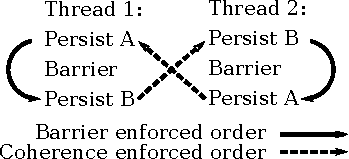
\includegraphics[width=.45\linewidth]{Persistency/cycle.pdf}
  \caption{\textbf{Cache Coherence Ordered Persists.} Thread 1's store visibility reorders while still attempting to enforce persist order.  The resulting persist order cycle is resolved by violating cache coherence persist order or by preventing stores from reordering across persist barriers.}
  \label{fig::Cycle}
\end{figure}


The example in Figure~\ref{fig::Cycle} demonstrates that it is not possible to simultaneously (1) allow store visibility to reorder across persist barriers, (2) enforce persist barriers, and (3) enforce persist order to a single address according to the order cache coherence observes those stores.
The example considers two distinct persistent objects, A and B.
Threads 1 and 2 persist to these objects in different program orders.
Thread 1's execution reorders the visibility of stores, while Thread 2 executes its stores in program order.
Note that the persist barrier implies that thread 1's persist to B occurs after its persist to A, but the values produced by these operations may become visible to other processors out of program order.

Figure~\ref{fig::Cycle} additionally annotates the persist order constraints (happens-before relationships) due to persist barriers and cache coherence store order.
As shown, these constraints form a cycle and hence cannot be enforced.
The cycle can be resolved by either coupling persist and store barriers---every persist barrier also prevents store visibility from reordering---or relaxing cache coherence persist order and providing additional mechanisms to order persists across threads.
It remains unclear how to best solve this dilemma.
Hence, for the remainder of this study, I focus on developing persistency models for SC.

\section{Conclusion}
\label{sec:Persistency:Conclusion}

Existing memory systems lack mechanisms to describe and enforce the order of persists.
I introduce memory persistency to explore the design space of interfaces and semantics for persistent memory.
Memory persistency builds on memory consistency to determine the values for and order of persist operations.
Memory persistency may be strict, relying on the consistency model to provide both thread and persist synchronization, or relaxed, decoupling thread synchronization from persist order and requiring additional persist barriers.
The next chapter introduces three persistency models and details their expected performance using a thread-safe persistent queue.
